%% 7.5 %%

\section{The Fundamental Theorem of Calculus}
\setcounter{exercise}{0}

\bx{
If $f$ is continuous, then we know from Theorem 7.2.9
that is is integrable. 

Then, from the Fundamental Theorem of Calculus,
that we can define
\begin{equation*}
  F(x) = \int_a^x f,
\end{equation*}
where $F'(c) = f(c)$ at all the continuous points of $f$.
This means $f$ is the derivative of $F$.
}

\bx{
\ea{
\item For $x \in [-1, 0]$, we just have 
\begin{equation*}
  F(x) 
  = \frac{
    (-x+1)(x+1)
  }{2}
  = \frac{
    1-x^2
  }{
    2
  }
\end{equation*}
For $x \in (-\infty, 1)$, 
\begin{equation*}
  F(x) = \int_{-1}^x f(x)
  = -\int_x^{-1} f(x) =
  -\frac{
    (1-x)(-1-x)
  }{
    2
  }
  = \frac{
    1-x^2
  }{
    2
  }
\end{equation*}
and for 
$x \in (1, \infty)$, we have 
\begin{equation*}
  F(x) = \frac{1}{2} + \frac{x^2}{2}
\end{equation*}
Putting these together gives 
\begin{equation*}
  F(x) = \begin{cases}
    \frac{1-x^2}{2}, &x \leq 0\\
    \frac{1+x^2}{2}, &x \geq 0
  \end{cases}
\end{equation*}
See Figure 
\ref{chap7:fig:Fx_final}
for the plot of $F(X)$.

I computed these by geometrically looking at the area of a trapezoid.
See Figure
\ref{chap7:fig:calculating_integral}
for more details.

\begin{figure}[H]
  \centering
  \subfloat[Finding $F(x)$]{
    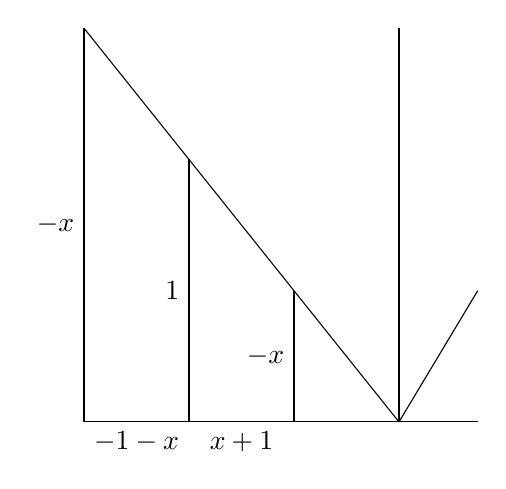
\begin{tikzpicture}
      \draw 
        (0,0) -- (0, 5)
        (0,0) -- (1, 0)
        (0,0) -- (-4, 0)
      ;

      \draw
        (0,0) -- (-4, 5)
        (0,0) -- (1, 5/3)
      ;

      \draw 
        (-4, 0) -- (-4, 5)
        (-8/3, 0) -- (-8/3, 10/3)
        (-4/3, 0) -- (-4/3, 5/3)
      ;

      \draw 
        (-4, 2.5) node[left] {$-x$}
        (-8/3, 5/3) node[left] {1}
        (-4/3, 5/6) node[left] {$-x$}
      ;

      \draw
        (-10/3, 0) node[below] {$-1-x$}
        (-2, 0) node[below] {$x+1$}
      ;
    \end{tikzpicture}
    \label{chap7:fig:calculating_integral}
  }
  \qquad
  \subfloat[$F(x)$]{
    \begin{tikzpicture}
      \begin{axis}[
          axis lines = center,
          xlabel = $x$,
          ylabel = {$F(x)$},
      ]

      \addplot[
          domain=0:3, 
          samples=100
      ]{
        0.5*x^2 + 1/2
      };

      \addplot[
          domain=-3:0, 
          samples=100
      ]{
        -0.5*x^2 + 1/2
      };
      \end{axis}
    \end{tikzpicture}
    \label{chap7:fig:Fx_final}
  }
  \caption{}
\end{figure}

$F$ is continuous everywhere, and differentiable everywhere.
Therefore, $F'(x) = f(x)$ everywhere as well.

\item 
\begin{figure}[H]
  \centering
  \subfloat[Finding $F(x)$]{
    \begin{tikzpicture}
      \begin{axis}[
          axis y line=middle, 
          axis x line=bottom,
          xlabel = $x$,
          ylabel = {$f(x)$},
          xticklabels={,$x_3$,,$-1$,$x_2$,,$x_1$,},
          ymin = 0,
          ymax = 3
      ]

      \addplot[
          domain=-3:0, 
          samples=10
      ]{
        1
      };

      \addplot[
          domain=0:3, 
          samples=10
      ]{
        2
      };

      \draw[dashed]
        (axis cs:-1, 0)
        -- (axis cs:-1, 3)
      ;

      \filldraw[pattern=horizontal lines]
        (axis cs:-3, 0)
        rectangle
        (axis cs:-1, 1)
      ;

      \filldraw[pattern=dots]
        (axis cs:-1, 0)
        rectangle
        (axis cs:0, 1)
      ;

      \filldraw[pattern=vertical lines]
        (axis cs:0, 0)
        rectangle
        (axis cs:2, 2)
      ;
      \end{axis}
    \end{tikzpicture}
    \label{chap7:fig:calculating_integral_b}
  }
  \qquad
  \subfloat[$F(x)$]{
    \begin{tikzpicture}
      \begin{axis}[
          axis lines = center,
          xlabel = $x$,
          ylabel = {$F(x)$},
      ]

      \addplot[
          domain=-3:-1,
          samples=10
      ]{
        x+1
      };

      \addplot[
          domain=-1:0,
          samples=10
      ]{
        x+1
      };

      \addplot[
          domain=0:3,
          samples=10
      ]{
        2*x+1
      };
      \end{axis}
    \end{tikzpicture}
    \label{chap7:fig:Fx_final_b}
  }
  \caption{}
\end{figure}

We can see from Figure 
\ref{chap7:fig:calculating_integral_b}
that we have 3 cases, $x_3 \in (-\infty, -1), x_2 \in [-1, 0], x_1 \in (0, \infty)$,
\begin{equation*}
  F(x) = \begin{cases}
    -(-1-x) \cdot 1, &x \leq -1\\
    (x-(-1)) \cdot 1, &x \in [-1, 0]\\
    1 + x \cdot 2, &x \geq 0
  \end{cases} \Rightarrow
  F(x) = \begin{cases}
    x+1, &x \leq 0\\
    2x+1, &x \geq 0
  \end{cases}
\end{equation*}

From Figure 
\ref{chap7:fig:Fx_final_b}
we see that 
$F$ is continuous everywhere, and but not differentiable at $x=0$,
since there is a kink.
However, we still have $F'(x) = f(x)$ everywhere,
thanks to the Fundamental Theorem of Calculus.
}
}

\bx{
We only need $F'(x) = f(x)$ for $x$ over $(a, b)$, since we 
are applyin the MVT.
}

\bx{
\ea{
\item We can compute 
\begin{equation*}
  H(1) = \int_1^1 \frac{1}{t} \dd{t} = 0
\end{equation*}
We know $1/t$ is differentiable over $t > 0$, so by the FTC
\begin{equation*}
  H'(x) = \frac{1}{x}
\end{equation*}

\item We have for $0 < x < y$
\begin{equation*}
  H(y) - H(x) 
  = 
  \int_{1}^y \frac{1}{t} \dd{t} -
  \int_{1}^x \frac{1}{t} \dd{t}\\
  =
  \int_{x}^y \frac{1}{t} \dd{t}\\
  > 0
\end{equation*}
Since $1/t > 0$ for $t > 0$, and we are finding its area over $[x, y]$.

\item We observe that 
\begin{align*}
  H'(cx) 
  &= c \cdot \frac{1}{cx} 
  = \frac{1}{x} 
  = H'(x) 
  = H'(x) + H'(c)\tag{$H'(c) = 0$ since $c$ constant}\\
  \int_1^x H'(ct) \dd{t} &=
  \int_1^x H'(t) \dd{t} +
  \int_1^x H'(c) \dd{t}\\
  H(cx) &=
  H(x) +
  H(c)
\end{align*}
}
I think the point of this exercise is to point out that 
with the properties shown, $\ln$ satisfies all of them,
so we can conclude that $H(x) = \ln(x)$.
}

\bx{
We can use Theorem 7.4.4 to show that 
since $f'_n \to g$ uniformly, and each $f'_n$ is integrable,
so we get 
\begin{align*}
  \lim_{n\to\infty} \int_a^x f'_n &= \int_a^x g\\
  \lim_{n\to\infty} f_n(x) - f_n(a) &= \int_a^x g\\
  f(x) - f(a) &= \int_a^x g\tag{$f_n \to f$}
\end{align*}
Now, we know $g$ is continuous on $[a, b]$, since $f'_n$ are all continuous,
so we can use the FTC to conclude that 
\begin{equation*}
  f'(x) = g(x)
\end{equation*}
}

\bx{
A missing assumption is that $f$ is continuous.
This is important, because if we now define 
\begin{equation*}
  G(x) = \int_a^x f,
\end{equation*}
we now know that $G$ is differentiable, so 
$G'(x) = f(x)$. We are given that $F(x)$ satisfies $F'(x) = f(x)$,
so combining,
\begin{equation*}
  G'(x) = f(x) = F'(x)
\end{equation*}
and we have that $G'(x) = F'(x)$.
Now, this is useful, since we know that this implies 
\begin{equation*}
  G(x) = F(x) + k.
\end{equation*} 
Finally, notice that $G(a) = 0 = F(a) + k$, so $k = - F(a)$.

We can now compute 
\begin{equation*}
  \int_a^b f = G(b) = F(b) - F(a)
\end{equation*}
}

\bx{
We can use FTC to show $\exists G, G'(x) = g(x)$, and
\begin{equation*}
  \frac{1}{b-1} \int_a^b g = 
  \frac{1}{b-a}\pbra{G(b) - G(a)}
\end{equation*}
Now by the MVT, we can conclude 
\begin{equation*}
  \exists c \in (a, b), G'(c) = 
  \frac{1}{b-a}\pbra{G(b) - G(a)}.
\end{equation*}
Finally, $G'(c) = g(c)$, so 
\begin{equation*}
  g(c) =
  G'(c) = 
  \frac{1}{b-a}\pbra{G(b) - G(a)} = 
  \frac{1}{b-1} \int_a^b g
\end{equation*}
}

\bx{
\ea{
\item We can write
\begin{align*}
  V\,f 
  &=
  \sup \pbrac{
    \sum_{k=1}^n
    \abs{
      f(x_k) - f(x_{k-1})
    }
  }\\
  &=
  \sup \pbrac{
    \sum_{k=1}^n
    \abs{
      \int_{x_{k-1}}^{x_k} f'
    }
  }\\
  &=
  \pbrac{
    \abs{
      \int_a^b f'
    }
  } \tag{Endpoints are $a, b$}\\
  &\leq 
  \int_a^b \abs{
    f'
  }
\end{align*}

\item With the MVT, we can show 
\begin{align*}
  V\,f 
  &=
  \sup \pbrac{
    \sum_{k=1}^n
    \abs{
      f(x_k) - f(x_{k-1})
    }
  }\\
  &=
  \sup \pbrac{
    \sum_{k=1}^n
    \abs{
      \frac{
        f(x_k) - f(x_{k-1})
      }{
        x_k - x_{k-1}
      } (x_k - x_{k-1})
    }
  }\\
  &=
  \sup \pbrac{
    \sum_{k=1}^n
    \abs{
      f(c'_k)
    }\Delta x_k
  }\\
  &= L(\abs{f'}, P_{\sup})\tag{Since $\abs{f(c'_k) \geq \inf \abs{f(x)}}$}\\
  &\leq L(\abs{f'}, P) = \int_a^b \abs{f'}
\end{align*}
We could have alternatively said
we know it is $= U(\abs{f'}, P)$, for some $P$,
which must be $\geq U(\abs{f'}) = \int_a^b \abs{f'}$.
}
}

\bx{
We see $U(h) = L(h) = b$ for $x \in [0, b]$, so $h$ is integrable.

We also can see that $H(x) = x$, so $H$ is differentiable at $x=1$.
}

\bx{
We can show $F(x)$ is not differentiable at $x=c$ by 
showing that $F'(c)$ equals different values depending on 
how we take the limit.

We'll show $F'(c) \to L_1 = \lim_{x \to c^-} f(x)$,
and a similar argument can be made for 
$F'(c) \to L_2 = \lim_{x \to c^+} f(x)$.

\begin{align*}
  \abs{
    F'(c) - L_1
  } 
  &= \abs{
    \lim_{x\to c^-} \frac{
      F(x) - F(c)
    }{
      x-c
    } - L_1
  }\\
  &= \abs{
    \frac{
      1
    }{x-c}
    \int_c^x \pbra{
      f(t) - 
      L_1
    }\dd{t}
  }
\end{align*}
Now, we can find 
\begin{equation*}
  t', \abs{f(t') - L_1} < \frac{\epsilon}{2}
\end{equation*}
We can also find 
\begin{equation*}
\delta, \abs{x - c} \Rightarrow 
\abs{f(x) - f(t')} < \frac{\epsilon}{2}
\end{equation*}
Then, 
\begin{align*}
  \abs{
    \frac{
      1
    }{x-c}
    \int_c^x \pbra{
      f(t) - 
      L_1
    }\dd{t}
  }
  &= \frac{1}{x-c}
  \int_c^x \abs{f(t) - f(t')} + \abs{f(t') - L_1}
  \dd{t}\\
  &\leq \frac{1}{x-c} 
  \int_c^x \pbra{
    \frac{\epsilon}{2} + \frac{\epsilon}{2}
  }
  \dd{t}\\
  &= \frac{1}{x-c} (x-c) \epsilon = \epsilon
\end{align*}

A similar argument occurs for $\lim_{x\to c^+} F'(c) = L_2$
And since $L_1 \neq L_2$, we conclude $F'(c)$ does not exist.

\label{chap7:ex:jump_disc_not_diff}
} 

\bx{
If we take $h(x)$ from Exercise
\ref{chap6:ex:_rational_monotone_continuous},
we see there is a discontinuity at every rational $r_n$,
since $u_n(x)$ contributes a jump at $r_n$ of $1/2^n$.

Now define $H(x) = \int_a^x h(x)$ for some $[a, b]$.
From Exercise
\ref{chap7:ex:jump_disc_not_diff},
we know that since $h(x)$ has a jump discontinuity at 
every $r_n$, we conclude $H(x)$ is not differentiable
at any $r_n$, which is $\mathbb{Q}$ and dense.

We still need to show that $H(x)$ is continuous and 
monotonic.

$H(x)$ is monotonic since $h(x) > 0$, over any nonzero interval,
so any $y>x$,
\begin{equation}
  H(y) - H(x) = \int_x^y h(t) \dd{t} > 0
\end{equation}
We can show $H(x) - H(c)$ is continuous, because 
given any $\epsilon > 0$,
choose $n$ such that 
\begin{equation*}
  2 \cdot \frac{1}{2^n} < \epsilon
\end{equation*}
The reason we have this condition is that 
in the worst case, we have an infinite number of 
$r_n$ near $H(c)$, which means the difference of 
\begin{equation*}
  \abs{
    H(x) - H(c)
  } \leq 
  \frac{1}{2^n} +
  \frac{1}{2^{n+1}} +
  \frac{1}{2^{n+2}} + \cdots
  \leq 2 \cdot
  \frac{1}{2^n}
\end{equation*}
Then choose a radius $\delta$ around $c$ 
such that there only exists $r_m$ with $m > n$.
This is always possible, since there are a finite 
number of $r_m$ such that $r_m \geq n$.

Then 
\begin{equation*}
  \abs{
    H(x) - H(c)
  } \leq 2 \cdot \frac{1}{2^n} < \epsilon
\end{equation*}
}